\setcounter{rownumber}{0}
\chapter{Manuscript I: Laser cooling of traveling wave phonons in an optical fiber}
\label{ch:Cooling}
\acresetall

\textit{This chapter elaborates on experiments and results related to optomechanical cooling, which have been published as an article of the same name in Physical Review Applied by Johnson et al. (2023) \cite{johnson2023laser}. Any discrepancies, omissions, or errors that may exist between the published paper and this dissertation chapter are the sole responsibility of the author, as the text, analyses, and interpretations herein represent an independent and original presentation of the work.}

%--------------------------------------------------------------------%

\section{Introduction}
\label{sec:Cooling:Introduction}

Materials above the ground state experience therodynamic variations such as temperature and density. These thermal fluctuations alter the optical properties of a given material, allowing a scattering process to occur (see Section \ref{sec:Introduction:Light-Scattering}).  Spontaneous Brillouin scattering is the inelastic scattering of light with these thermal fluctuations within a material, facilitating an energy exchange between the optical and acoustic domains. While a given medium typically supports a multitude of thermally excited acoustic modes (including both transverse and longitudinal modes) we focus here specifically on longitudinally travelling acoustic waves.

%--------------------------------------------------------------------%

\section{Optomechanical Cooling and Heating}
\label{sec:Cooling:Cooling-Heating}

Backward Brillouin scattering targets these longitudinally traveling acoustic waves (or phonons) through two complementary processes---Stokes and anti-Stokes, illustrated in Figures \ref{fig:Cooling:StokesHeating} and \ref{fig:Cooling:anti-StokesCooling}, respectively. In the Stokes process, an incident photon of frequency \(\omega\) scatters with a \textit{retreating} phonon of frequency \(\Omega\) annihilating the \textit{photon} and creating both an additional phonon of frequency \(\Omega\) and a backscattered photon at the difference energy (\(\omega_{\mathrm{Stokes}} = \omega - \Omega\)). In this way, both energy and momentum are conserved. This can be visualized by an analogy, in which the incident light experiences a doppler \textit{down}-shift in frequeny as though the photon were reflected from a retreating mirror. Since this processes results in an increase in the phonon population within the respective longitudinal mode of the material, this process is referred to as optomechanical heating. The energy lost by the light is gained by the material in the form of mechanical vibrations.

% \begin{figure}[t] % here (h), at the top (t), at the bottom (b), or on a separate page for floats (p), in that preference order
% \centering
% 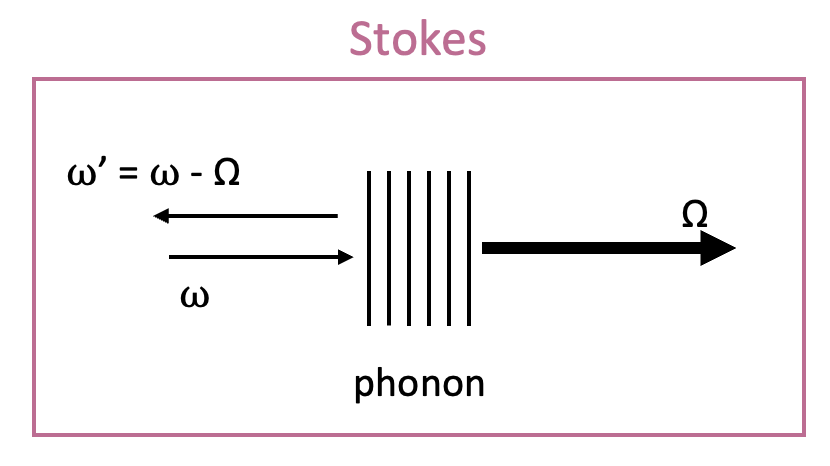
\includegraphics[width=\textwidth]{figs/3-Cooling/StokesHeatingProcess.png}
% \caption{}
% \label{fig:Cooling:StokesHeating}
% \end{figure}
%
% \begin{figure}[h] % here (h), at the top (t), at the bottom (b), or on a separate page for floats (p), in that preference order
% \centering
% 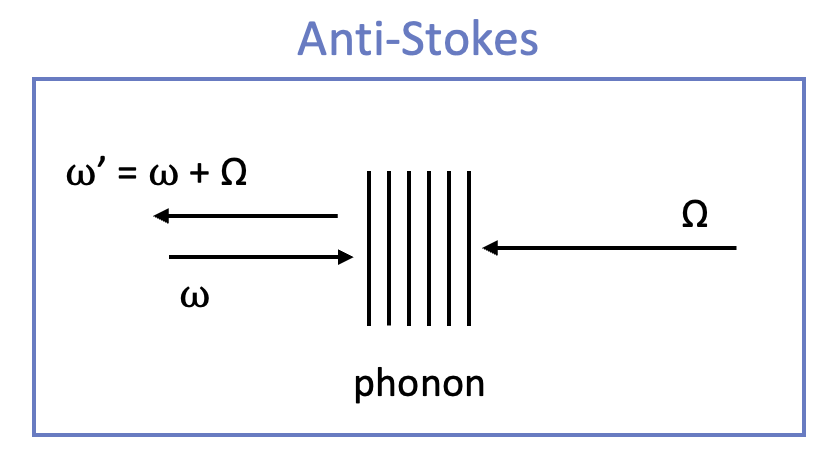
\includegraphics[width=\textwidth]{figs/3-Cooling/anti-StokesCoolingProcess.png}
% \caption{}
% \label{fig:Cooling:StokesCooling}
% \end{figure}

\begin{figure}[t]
    \centering
    \begin{subfigure}[b]{0.49\textwidth}
        \centering
        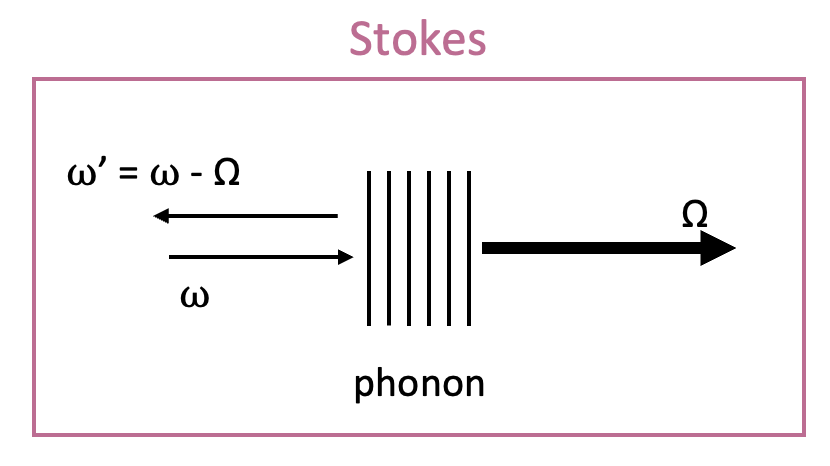
\includegraphics[width=\textwidth]{figs/3-Cooling/StokesHeatingProcess.png}
        \caption{}
        \label{fig:Cooling:StokesHeating}
    \end{subfigure}
    \hfill
    \begin{subfigure}[b]{0.49\textwidth}
        \centering
        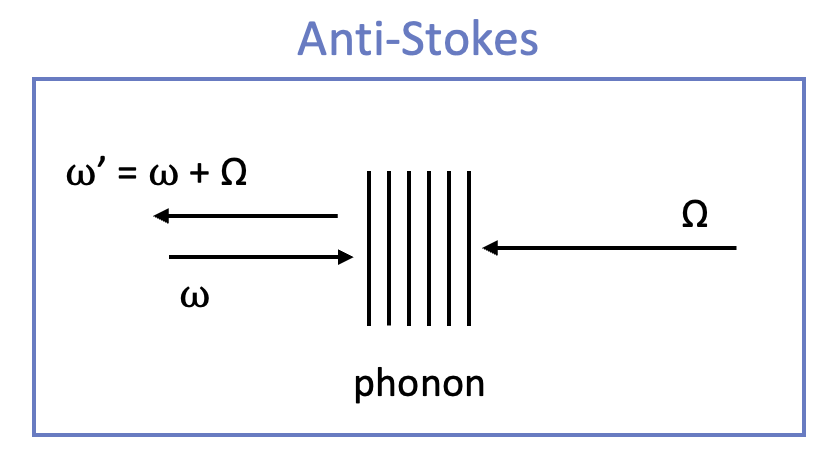
\includegraphics[width=\textwidth]{figs/3-Cooling/anti-StokesCoolingProcess.png}
        \caption{}
        \label{fig:Cooling:anti-StokesCooling}
    \end{subfigure}
    \caption{Illustration of optomechanical heating and cooling processes. Figure \ref{fig:Cooling:StokesHeating} shows an incident photon of frequency \(\omega\) scattering with a retreating phonon of frequency \(\Omega\), resulting in the annihilation of the incident photon and the creation of both an additional retreating phonon of frequency \(\Omega\) and a backwards propagating photon of reduced frequency and thereby energy (\(\omega_{\mathrm{Stokes}} = \omega - \Omega\)). Figure \ref{fig:Cooling:anti-StokesCooling} shows the inverse process, whereby an incident photon, \(\omega\), scatters with an approaching phonon, \(\Omega\), annihilating the incident photon and the phonon to produce a backwards propagating photon of increased frequency and thereby energy (\(\omega_{\mathrm{anti-Stokes}} = \omega + \Omega\)).}
    \label{fig:Cooling:StokesProcesses}
\end{figure}

The anti-Stokes process is the inverse process, whereby an \textit{approaching} phonon of frequency \(\Omega\) scatters with an incident photon of frequency \(\omega\), annihilating the \textit{phonon} and creating a backscattered photon at the addition energy (\(\omega_{\mathrm{anti-Stokes}} = \omega + \Omega\)). Both energy and momentum are again conserved, however in the anti-Stokes process, the incident light experiences a doppler \textit{up}-shift in frequency as if, to continue the analogy, the photon were reflected from an approaching mirror. For further intuition, one might consider an elastic collision of a ball (the photon) with a moving wall (the phonon) for the cases of the wall moving towards (anti-Stokes process) and away (Stokes process) from the ball as they collide. This simple analogy helps illustrate how momentum and energy are exchanged in optomechanical heating (Stokes) and cooling (anti-Stokes) processes.

%--------------------------------------------------------------------%

\section{Cooling Platform: \texorpdfstring{$CS_{2}$}{CS2}-Liquid Core Optical Fiber}
\label{sec:Cooling:Platform}

Demonstration of optomechanical cooling and heating of traveling wave phonons requires a device or material host that [can balance all of the requirements I just layed out in the previous section!] features large optomechanical coupling as well as tight optical and acoustic confinement for large acousto-optic overlap.  a \ce{CS2}-filled \ac{LCOF} similar to that used by Behunin et al. (2019). \cite{behunin2019spontaneous}

\subsection{Optomechanical Properties}
\label{subsec:Cooling:Platform:Properties}


\subsection{Fabrication}
\label{subsec:Cooling:Platform:Fabrication}

Fabrication of the \ce{CS2}-\ac{LCOF} was performed with a Vytran fusion splicing workstation.


\subsection{Fabrication Iterative Refinement}
\label{subsec:Cooling:Platform:Refinement}

%--------------------------------------------------------------------%

\section{Intention of the Pump-Probe Experiment}
\label{sec:Cooling:Intention}

%--------------------------------------------------------------------%

\section{Experimental Setup}
\label{sec:Cooling:Setup}


\subsection{Main Experiment}
\label{subsec:Cooling:Setup:Main}


\subsection{Pump-Probe Experiment}
\label{subsec:Cooling:Setup:Pump-Probe}

%--------------------------------------------------------------------%

\section{Results}
\label{sec:Cooling:Results}


\subsection{Main Experiment Results}
\label{subsec:Cooling:Results:Main}


\subsection{Pump-Probe Experiment Results}
\label{subsec:Cooling:Results:Pump-Probe}

%--------------------------------------------------------------------%

\section{Discussion}
\label{sec:Cooling:Discussion}


\subsection{Application to Ground State Cooling}
\label{subsec:Cooling:Discussion:Ground-State}


\subsection{Standardized Cooling Metric}
\label{subsec:Cooling:Discussion:Metric}


\subsection{Tapered chalcogenide Photonic Crystal Fiber: Max Plank Results}
\label{subsec:Cooling:Discussion:Max-Plank}
